\documentclass{article}
\usepackage{amsmath, amssymb}
\usepackage{graphicx}
\usepackage{caption}
\usepackage{tikz}
\usepackage{geometry}
\geometry{margin=1in}


\title{Research Methodology Practical Test}
\author{B.Sc(H) Mathematics – Semester VI}
\date{}

\begin{document}

\maketitle

\section*{Answer 1: Typeset Mathematical Expressions}

(a)
\[
F(x, y) = \int_{-\infty}^{y} \int_{-\infty}^{x} e^{-x^2 - y^2} \, dx \, dy
\]

(b)
\[
1 + \tan^2x = 1 + \frac{\sin^2x}{\cos^2x} = \frac{\sin^2x + \cos^2x}{\cos^2x} = \frac{1}{\cos^2x} = \sec^2x
\]

(c)
\[
\left| \begin{array}{ccc}
1 & 3 & 5 \\
0 & 4 & 6 \\
0 & 0 & 34 \\
\end{array} \right| = 136
\]

\section*{Answer 2: Create Table in LaTeX}

\begin{table}[h!]
\centering
\begin{tabular}{|c|l|l|c|}
\hline
\textbf{Sr.No.} & \textbf{Student Name} & \textbf{College Name} & \textbf{CGPA} \\
\hline
1 & DUMH0001 & Miranda House & 9 \\
2 & DUSRCC0002 & SRCC & 8.5 \\
3 & DUDRC00034 & DRC & 9 \\
4 & DUSTPH000321 & St. Stephen & 9 \\
5 & DUHRC000134 & Hansraj College & 8.9 \\
6 & DUSVC000134 & SVC & 8.79 \\
\hline
\end{tabular}
\caption{Student CGPA Information}
\end{table}

\section*{Answer 3: More Expressions}

\subsection*{(a) Series Notation}
\[
a_1 + a_2 + \dots + a_n = a_1 + a_2 + \ldots + a_n
\]

\subsection*{(b) Set Product Distribution}
\[
A \times \left( \bigcup_{i=1}^{n} B_i \right) = \bigcup_{i=1}^{n} (A \times B_i)
\]

\subsection*{(c) Decorated Sum Expression}
\[
\underbrace{1 + 3 + \dots + 99}_{\text{odd numbers}} 
+ \underbrace{2 + 4 + \cdots + 100}_{\text{even numbers}} 
= \underbrace{1 + 2}_{\text{first pair}} 
+ \underbrace{3 + 4 + \dots + 97 + 98}_{\text{middle terms}} 
+ \underbrace{99 + 100}_{\text{last pair}}
\]

\section*{Answer 4: Plot the Diagram}

\begin{center}
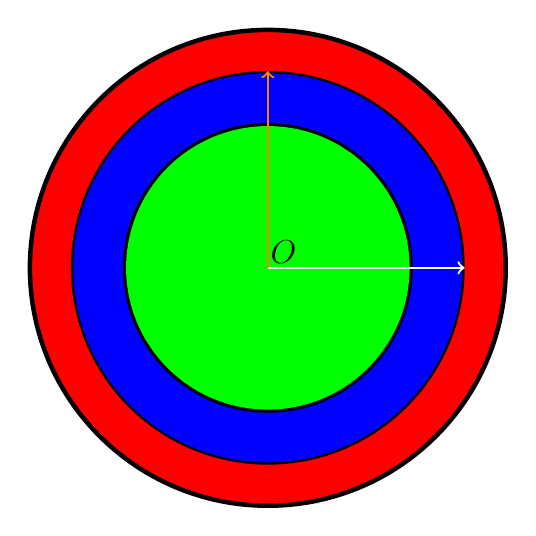
\begin{tikzpicture}
% Red outer ring
\fill[black] (0,0) circle (3.05);
\fill[red] (0,0) circle (3);
\fill[black] (0,0) circle (2.5);
\fill[blue] (0,0) circle (2.47);
\fill[black] (0,0) circle (1.84);
\fill[green] (0,0) circle (1.8);

% Axes arrows
\draw[->, white, thick] (0,0) -- (2.5,0); % x-axis
\draw[->, orange, thick] (0,0) -- (0,2.5); % y-axis

% Origin label
\node at (0.2,0.2) {\large $O$};

% Outline circle
\draw (0,0) circle (3);
\end{tikzpicture}
\end{center}



\section*{Answer 5: Plot $y = \sin x + x^2$}

\begin{center}
\begin{tikzpicture}[scale=0.7]
\draw[->] (-5, 0) -- (5, 0) node[right] {x};
\draw[->] (0, -5) -- (0, 20) node[above] {y};
\draw[domain=-4:4, smooth, variable=\x, blue, thick] plot ({\x}, {sin(\x r) + \x*\x});
\node at (2,10) {$y = \sin x + x^2$};
\end{tikzpicture}
\end{center}

\end{document}
